\documentclass[18pt, twoside]{article}
\usepackage[utf8]{inputenc}
\usepackage{polski}
\usepackage{graphicx}
\graphicspath{ {./images/} }
\usepackage[margin=0.5in]{geometry}


\begin{document}
\begin{figure}[tp!]
\center{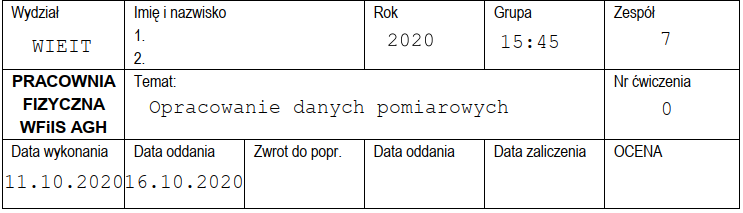
\includegraphics{F}}
\end{figure}

\begin{center}
    \section*{Opracowanie Danych Pomiarowych}
    \emph{Dzmitry Mikialevich}
\end{center}
\begin{center}
    \emph{Wojciech Sikora}
\end{center}
\tableofcontents
\newpage

\section{Wstęp}
\subsection{Cel ćwiczenia}
 % Tu TEKST
\subsection{Opis ćwiczenia}
 % Tu TEKST
\section{Układ Pomiarowy}
 % Tu TEKST
\section{Przebiegi doświadczenia}
 % Tu TEKST
\section{Wyniki Pomiarów}

Długość wahadła - \[l= 45 cm = 450 mm \]\newline
Niepewność pomiaru - \( ? \)
{
     \begin{table}[h]
     \centering
    \begin{tabular}{|l|l|l|l|}
    \hline

    Lp.& Liczba okresów k & Czas t dla k okresów \([s]\)  & okres \(T_i = t/k \)  \([s]\)   \\ \hline
    1 & 10  & 13,22 & 1,322 \\ \hline
2 & 10  & 13,62 & 1,362 \\ \hline
3 & 10  & 13,92 & 1,392 \\ \hline
4 & 10  & 13,37 & 1,337 \\ \hline
5 & 10  & 13,38 & 1,338 \\ \hline
6 & 10  & 13,28 & 1,328 \\ \hline
7 & 10  & 13,34 & 1,334 \\ \hline
8 & 10  & 13,35 & 1,335 \\ \hline
9 & 10  & 13,37 & 1,337 \\ \hline
10 & 10  & 13,45 & 1,345 \\ \hline
    \end{tabular}
    \textbf{\caption{Pomiar okresu drgań przy ustalonej długości wahadła  }
}
\end{table}}


{
     \begin{table}[h]
     \centering
    \begin{tabular}{|l|l|l|l|l|l|}
    \hline
    Lp. & l \([mm]\) & \(k\) & \(t[s]\) & \(T_i[s]\) &  \(T_i^2[s^2]\) \\ \hline
    1 & 280  & 10 & 10,23 & 1,023 & 1,046529 \\ \hline
2 & 300  & 10 & 11,3 & 1,13 & 1,2769 \\ \hline
3 & 310  & 10 & 11,72 & 1,172 & 1,373584 \\ \hline
4 & 330  & 10 & 12,22 & 1,222 & 1,493284 \\ \hline
5 & 340  & 10 & 12,35 & 1,235 & 1,525225 \\ \hline
6 & 350  & 10 & 12,41 & 1,241 & 1,540081 \\ \hline
7 & 360  & 10 & 12,52 & 1,252 & 1,567504 \\ \hline
8 & 370  & 10 & 12,71 & 1,271 & 1,615441 \\ \hline
9 & 400  & 10 & 12,96 & 1,296 & 1,679616 \\ \hline
10 & 440  & 10 & 13,11 & 1,311 & 1,718721 \\ \hline
11 & 450  & 10 & 13,31 & 1,331 & 1,771561 \\ \hline
12 & 480  & 10 & 14,42 & 1,442 & 2,079364 \\ \hline
13 & 500  & 10 & 14,43 & 1,443 & 2,082249 \\ \hline
14 & 520  & 10 & 14,71 & 1,471 & 2,163841 \\ \hline
15 & 550  & 10 & 15,7 & 1,57 & 2,4649 \\ \hline
    \end{tabular}
    \textbf{\caption{Pomiar zależności okresu drgań od długości wahadła }
}
\end{table}}
 

 
 
 
\section{Opracowanie wyników Pomiarów}
\subsection{Błędy grube}
\textbf{Zadanie:} Oceń, czy wyniki pomiaru okresu nie zawierają błędów grubych. (Zwrócić uwagę na największą 
 i najmniejszą wartość Ti w uzyskanym zestawie danych)\newline
Przy analizie wyników nie zauważyliśmy błędów grubych. Różnica między największą a najmniejszą wartością wynosi \[\Delta t = t_{max} - t_{min} = ?? \]
\subsection{Niepewność pomiaru okresu (typu A)}
\textbf{Zadanie:} Oblicz niepewność pomiaru okresu (typu A). \newline
\[u(T) =\sqrt{\frac{\sum{(T_i - \overline T)^2}}{n(n-1)}} = ??\] gdzie:  \(\overline T\) - średni okres, \(T_i\) - okres zmierzony zai-tym razem, n - liczba pomiarów
 \subsection{Niepewność pomiaru długości wahadła (typu B)}
\textbf{Zadanie:} Oceń niepewność pomiaru długości wahadła (typu B).\newline Podziałka linijki, za pomocą której było mierzone wahadło wynosi \(1mm\), jednak oszacowanie środka ciężkości stanowiło problem, dlatego oszacowaliśmy niepewność typu B jako \(5mm\)
 \subsection{Przyspieszenie ziemskie  na podstawie uzyskanych wartości \(l\) i \(T\)}
Korzystając ze wzoru na okres drgań wachadła matematycznego dla małych kątów odchylenia, mamy: \[T = 2\pi \sqrt{\frac{l}{g}} \Rightarrow g = \frac{4\pi^2}{T^2}l = \frac{4 \times 3.141^2}{(1.343s)^2} * 450mm = 9,859 m/s^2\]
 \subsection{Niepewność złożoną \(u_c(g)\) przy pomocy prawa przenoszenia niepewności}
\textbf{Zadanie:} Oblicz niepewność złożoną uc(g) przy pomocy prawa przenoszenia niepewności. \newline
\[u_c(g) = \sqrt{(\frac{\partial g}{\partial l} u(l))^2 + (\frac{\partial g}{\partial T} u(T))^2} = ?\]
 \subsection{Niepewność rozszerzoną \(U(g)\)) przy pomocy prawa przenoszenia niepewności}
\textbf{Zadanie:}Oblicz niepewność rozszerzoną U(g).\newline
\[U(g) = k \times u(g) = ?\]
BLA BLA BLA
 \subsection{Porównanie uzyskanej wartości przyspieszenia ziemskiego z wartością tabelaryczną}
 
%Wojciech PART
 
 % Tu TEKST
 \subsection{wykres zależności okresu od długości wahadła \(T(l)\)}
 % Tu TEKST
 \subsection{Wykres zlinearyzowany \(T^2\) w funkcji l}
 % Tu TEKST
 \subsection{Dopasowanie prostej typu \(y = ax\)}
 % Tu TEKST
 \subsection{Wartość przyspieszenia 
ziemskiego z otrzymanej wartości współczynnika nachylenia}
 % Tu TEKST
 \subsection{Obliczanie niepewności u(g) z niepewności u(a) }
 % Tu TEKST
\section{Wnioski}
\subsection{elo}
 % Tu TEKST

\end{document}